\section{Building Models}
\subsection{\M~ Dataset}
First the data must be load and turned into a \M~ dataset with the following commands. Here this is shown by the example of the pewee\_df data. 
\begin{verbatim}
data(pewee_df)
PEWEE <- march.dataset.loadFromDataFrame(pewee_df, 
                    				  MARGIN = 1, weights = NA, missingDataRep = NA)
\end{verbatim}•
If everything worked well it should be able to see the Data and the Values which are now a callable option for the different Markovian models as shown in  \refig{fig:data} for the example of the pewee\_df. 
\begin{figure}[h]
    \centering
    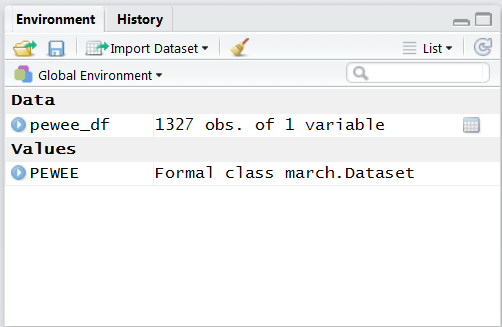
\includegraphics[scale=0.8]{dataset}
    \caption{Data and Values of the pewee\_df example}
    \label{fig:data}
\end{figure}
For a better explanation and several examples concerning load data from a Dataframe see the following help command. 
\begin{verbatim}
help(march.dataset.loadFromDataFrame)
\end{verbatim}•
\subsection{Building Homogenous Markov Chains Models}
Now all the preparations to start a markovian models are done. To start an example of the Independence Model is chosen. It calculates the loglikelihood, the total number or variables (dsl) aswell as the Aikake (AIC) and the Bayesian (BIC) Information Criterion. The outcome indP is the percentage for each of the variables. The model is built with the following command.
\begin{verbatim}
Indep <- march.indep.construct(PEWEE)
\end{verbatim}•
The Indep class should now appear in the environment window of your R-Studio, \refig{fig:data}.
Notice that the model is built with the \M~dataset! Further the results and a summary should be printed.
\begin{verbatim}
print(Indep)
march.summary(Indep)
\end{verbatim}•
Now the results should appear in the console of the R-Studio as it is shown for the pewee\_df example in \refig{fig:indep}.
\begin{figure}[h]
    \centering
    \includegraphics[scale=0.8]{indep}
    \caption{Results of the pewee\_df example}
    \label{fig:indep}
\end{figure}
Now the maxOrder parameter is used. With the output of the following commands it is obvious that the total amount of used variables (dsl) is reduced by the the value of maxOrder. The Independence Model needs the first 5 variables to create the model starting from the 6th variable.
\begin{verbatim}
Indep.2 <- march.indep.construct(PEWEE,maxOrder=5)
print(Indep.2)
\end{verbatim}•
To build Markov chains with the loaded data the following command is used. The first two examples are both first order and only differs in their value of the maximal order. 
\begin{verbatim}
MC1 <- march.mc.construct(y=PEWEE,order=1,maxOrder=1)
print(MC1)
MC1.2 <- march.mc.construct(PEWEE,order=1,maxOrder=5)
print(MC1.2)
\end{verbatim}•
With:\\
y: \hspace{37pt}   MARCH Dataset\\
order:\hspace{23pt}   order of the constructed Markov ChainYY\\
maxOrder:   \hspace{0pt}maximum visible order among the set of Markovian models to compare\newpage
\hspace*{-17pt}In the third example a Markov chain second order is created by \M.
\begin{verbatim}
MC2 <- march.mc.construct(PEWEE,order=2,maxOrder=5)
print(MC2)
\end{verbatim}•
Now the differences between 1st and 2nd order are visible. For more information about the construction of the independence model, the Markov chains (mc) or the summary of the results see:
\begin{verbatim}
help(march.indep.construct)
help(march.mc.construct)
help(march.summary)
\end{verbatim}•
as well as their description of the class: 
\begin{verbatim}
help("march.Indep-class")
help("march.Mc-class")
\end{verbatim}•
For further informations and a mathematical background explanation of Markov Chains see \cite{berchtold2002mixture}.
\subsection{Comparison of the Mixture Transition Distributions, High Order Markov Chains and the Independent Model}
In the next example a comparison between three different models with sleep data is built. Therefore the Indepence model is built first and then Markov chains of 1st to 3rd order. The maximal order of 3 is the same for every model. How the models are built and the results are saved in a list is shwon by the following commands.
\begin{verbatim}
models <- list()
models[[length(models)+1]] <- march.indep.construct(sleep,maxOrder=3)
models[[length(models)+1]] <- march.mc.construct(sleep,order=1,maxOrder=3)
models[[length(models)+1]] <- march.mc.construct(sleep,order=2,maxOrder=3)
models[[length(models)+1]] <- march.mc.construct(sleep,order=3,maxOrder=3)
\end{verbatim}•
To show the performance of the indicators like loglikelihood (ll), number of independent parameters (param), as well as the Bayesian (BIC) and the Aikake Information Criterion (AIC) it is necessary to bind all these informations together in a variable, here called r which then can be printed. 
\begin{verbatim}
r <- do.call(rbind,lapply(models,march.summary))
print(r)
\end{verbatim}•
The result should appear like shown in \refig{fig:IndepMC123}
\begin{figure}[h]
    \centering
    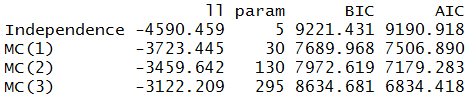
\includegraphics[scale=0.8]{IndepMC123}
    \caption{Summary of the informations about Independent Model and MC 1 to 3}
    \label{fig:IndepMC123}
\end{figure}
Further a Mixture Transition Distributions (MTD) models with different orders can be created with the following command.
\begin{verbatim}
mtd <- march.mtd.construct(y=march.Dataset, order, maxOrder )
\end{verbatim}•
For more information about the construction of the MTD models and a general description of MTD see the help pages.
\begin{verbatim}
help("march.mtd.construct")
help("march.Mtd-class")
\end{verbatim}•
These models are explained in \cite{berchtold2002mixture}.
Now a first example of the MTD models will be shown and the output shortly discussed. 
\begin{verbatim}
mtd2 <- march.mtd.construct(sleep,order=2,maxOrder=3)
print(mtd2)
march.summary(mtd2)
\end{verbatim}•
The output of the summary command are the transition matrix Q, the vector of lag parameters phi as well as the loglikelihood ll and the number of parameters dsL.\\ Now some more MTD models with different orders are created which later will be compared to the models calculated before. 
\begin{verbatim}
mtd3 <- march.mtd.construct(sleep,order=3,maxOrder=3)
print(mtd3)
march.summary(mtd3)

mtdg2 <- march.mtd.construct(sleep,order=2,maxOrder=3,mtdg=TRUE)
print(mtdg2)
march.summary(mtdg2)

mtdg3 <- march.mtd.construct(sleep,order=3,maxOrder=3,mtdg=TRUE)
print(mtdg3)
march.summary(mtdg3)
\end{verbatim}•
Now to compare all the different models calculated above a list which contains all the informations is created. Then the output of the command is the summary of all the models which now can be compared easily. 
\begin{verbatim}
models_all <- list(8)
models_all[1] <- models[1]
models_all[2] <- models[2]
models_all[3] <- models[3]
models_all[4] <- mtd2
models_all[5] <- mtdg2
models_all[6] <- models[4]
models_all[7] <- mtd3
models_all[8] <- mtdg3

r <- do.call(rbind,lapply(models_all,march.summary))
print(r)
\end{verbatim}•
In \refig{fig:sumMC} the summary of the results of the different models are shown. 
\begin{figure}[h]
    \centering
    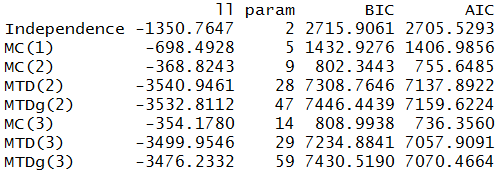
\includegraphics[scale=0.8]{sumMC}
    \caption{Summary of the different models}
    \label{fig:sumMC}
\end{figure}
With this summary it is detectable that in relation to the BIC the Markov Chain model 2nd order is the best. According to the AIC the Markov Chain model 3rd order is the best. To print detailled informations about a model the following command is necessary.
\begin{verbatim}
print(models[i])
\end{verbatim}•
Here i is the dummie variable of the location of the model inside the array list. For example the Independence model is in the first place of the list so the dummie variable is replaced by 1. 

\subsection{Building Hidden Markov Chain Model}
Now the hidden models are introduce and compared with the homogenous models already built. Here a introduction into two different Hidden models, the Hidden Markov Model and the Double Chain Markov model is given. First the data is loaded and a march.Dataset is created therefore several different homogenous models are built and compared, so the the best model can be found. The maximal order is set to 3. This is done with the following commands. 
\begin{verbatim}
data(pewee_df)
PEWEE <- march.dataset.loadFromDataFrame(pewee_df, 
                   MARGIN = 1, weights = NA, missingDataRep = NA)

models <- list()
models[[length(models)+1]] <- march.indep.construct(PEWEE,maxOrder=3)
models[[length(models)+1]] <- march.mc.construct(PEWEE,order=1,
										maxOrder=3)
models[[length(models)+1]] <- march.mc.construct(PEWEE,order=2,
										maxOrder=3)
models[[length(models)+1]] <- march.mc.construct(PEWEE,order=3,
										maxOrder=3)
models[[length(models)+1]] <- march.mtd.construct(PEWEE,order=2,
										maxOrder=3,llStop=0.0001)
models[[length(models)+1]] <- march.mtd.construct(PEWEE,mtdg=TRUE,order=2,
										maxOrder=3,llStop=0.0001)
models[[length(models)+1]] <- march.mtd.construct(PEWEE,order=3,
										maxOrder=3,llStop=0.0001)
models[[length(models)+1]] <- march.mtd.construct(PEWEE,mtdg=TRUE,order=3,
										maxOrder=3,llStop=0.0001)

r <- do.call(rbind,lapply(models,march.summary))
print(r)
\end{verbatim}•
Now a comparison between the different homogenous models can be made. According to the BIC, the Markov Chain Model second order fits the data best, because this model has the lowest BIC value as seen in \refig{fig:hmcSum}.   
\begin{figure}[h]
    \centering
    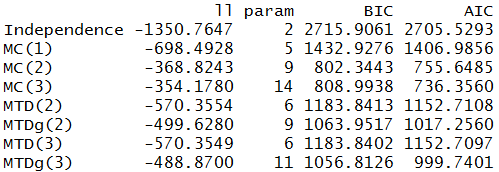
\includegraphics[scale=0.8]{hmcSum}
    \caption{Summary of the different models}
    \label{fig:hmcSum}
\end{figure}
Now to show more detailed informations about the best model we can print them with the following command.
\begin{verbatim}
print(models[3])
\end{verbatim}•
May with another march.Dataset another model will be the best. To print it, the right position of the models[] array needs to be written into the comman. To compare the best homogenous model with the Hidden Markov Models they need to be created first. \\
First the Hidden Markov model is created. For more general informations and informations about the construction of Hidden Markov models see these help commands. 
\begin{verbatim}
help(march.dcmm.construct)
help("march.Dcmm-class")
\end{verbatim}•
Now we want to create a Hidden Markovian Model therefore the following constructor is used. 
\begin{verbatim}
march.dcmm.construct(y, orderHC, orderVC, M, gen = 5, popSize = 4,
         maxOrder = orderVC, seedModel = NULL, iterBw = 2, stopBw = 0.1)
\end{verbatim}•
With\\
y: \hspace{44pt} is the march.Dataset\\
orderHC: \hspace{10pt} of the hidden chain\\ 
orderVC: \hspace{11pt} the order of the visible chain\\
M: \hspace{42pt} the number of hidden state\\
gen: \hspace{33pt} the number of generation performed by an evolutionary alglorithm\\ 
popSize: \hspace{13pt} the number of individuals stored into the population\\
maxOrder: \hspace{2pt} the maximum visible order among the set of Markovian models to compare\\
seedModel: \hspace{0pt} a model to optimize using Baum-Welch algorithm\\
iterBw: \hspace{18pt} the number of iteration performed by the Baum-Welch algorithm\\ 
stopBw: \hspace{15pt}  is the minimum increase in quality (log-likelihood) authorized in  the Baum- \hspace*{62pt}Welch algorithm\\
To build Hidden Markovian Models (HMM) with the command described above it is necessary to set the order of the visible chain to zero \mbox{(orderVC~=~0)}. With the following commands two HMM are built and one is printed. 
\begin{verbatim}
HMM.1 <- march.dcmm.construct(PEWEE,orderHC=1,M=2,orderVC=0,maxOrder=3,
                              popSize=10,gen=5)
march.summary(HMM.1)

HMM.2 <- march.dcmm.construct(PEWEE,orderHC=1,M=2,orderVC=0,maxOrder=3,
                              popSize=1,gen=1,iterBw=50,stopBw=0.0001)
march.summary(HMM.2)
\end{verbatim}•
This should get the output similar to what is visible in \refig{fig:hmm2} where the value in brackets in the first column is the order of the hidden chain (orderHC). 
\begin{figure}[h]
    \centering
    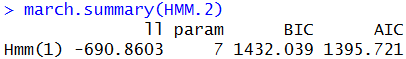
\includegraphics[scale=0.8]{hmm2}
    \caption{the summary of a Hidden Markovian Model first order}
    \label{fig:hmm2}
\end{figure}
To print further details about the model the print command is used. The help page to the Dcmm.class where the output is described is also useful. 
\begin{verbatim}
print(HMM.2)
help("march.Dcmm-class")
\end{verbatim}

\subsection{Building Double Chain Markov Model}
To create Double Chain Markov models (DCMM) the same constructor is used with which the HMM have been built already. But now the order of visible chains and hidden chain is set to greater than 0 so there is at least one hidden chain and one visible chain.
\begin{verbatim}
march.dcmm.construct(y, orderHC > 0, orderVC > 0, M, gen = 5, popSize = 4,
         maxOrder = orderVC, seedModel = NULL, iterBw = 2, stopBw = 0.1)
\end{verbatim}•
 For more informations and a detailled explanation of the DCMM as well as a detailed mathematical description read \cite {Berchtold2002}.
To create the first example of a DCMM the following code with one visible and one hidden chain is used. 
\begin{verbatim}
DCMM.1A <- march.dcmm.construct(PEWEE,orderHC=1,M=2,orderVC=1,maxOrder=3,
                               popSize=4,gen=5,iterBw=2,stopBw=0.0001)
print(DCMM.1)
\end{verbatim}
Now additional iterations should be calculated. Fot this the Baum Welch (BW) Algortihm is used and the number of iterations  is set to 50 (iterBw~=~50). The previous model is used as a seed Model. 
\begin{verbatim}
DCMM.1 <- march.dcmm.construct(PEWEE,orderHC=1,M=2,orderVC=1,maxOrder=3,
                               seedModel=DCMM.1A,iterBw=50,stopBw=0.0001)
print(DCMM.1)

march.summary(DCMM.1)
march.summary(DCMM.2)
\end{verbatim}•
In \refig{fig:dcmm_12} the comparison between these two different computation of a DCMM is shown. The name of the models is followed by the orders of the HC and VC in brackets, here for both models and both orders 1. It is obvious that with additional iterations the BIC as well as the AIC have improved. DCMM.1A is first calculated and DCMM.1 is calculated with additional BW iterations and the first model as a seed model.
\begin{figure}[h]
    \centering
    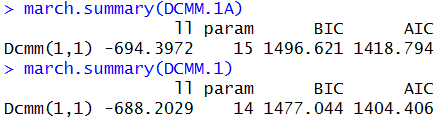
\includegraphics[scale=0.8]{dcmm_12}
    \caption{the summary of the two DCMM.}
    \label{fig:dcmm_12}
\end{figure}\\
In the next example the hidden states are raised, which is represented by the variable M.
\begin{verbatim}
DCMM.2 <- march.dcmm.construct(PEWEE,orderHC=1,M=3,orderVC=1,maxOrder=3,
                               popSize=1,gen=1,iterBw=50,stopBw=0.0001)
march.summary(DCMM.2)
\end{verbatim}•
A comparison between \refig{fig:dcmm_2} and \refig{fig:dcmm_12} shows the improvement of the AIC and the BIC. But with the higher number of parametres the computation time increases.
\begin{figure}[h]
    \centering
    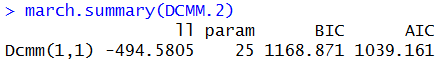
\includegraphics[scale=0.8]{dcmm_2}
    \caption{the summary of the DCMM with more hidden states.}
    \label{fig:dcmm_2}
\end{figure}\\
For the next example the hidden order is raised to 2 and the number of hidden states is reduced to the former value. 
\begin{verbatim}
DCMM.3 <- march.dcmm.construct(PEWEE,orderHC=2,M=2,orderVC=1,maxOrder=3,
                               popSize=1,gen=1,iterBw=50,stopBw=0.0001)
march.summary(DCMM.3)
\end{verbatim}•
In \refig{fig:dcmm_3} the improvement of BIC and AIC is visible as well as the reduction of the parametres. An improvement of the loglikelihood is done in comparison with the previous models.
\begin{figure}[h]
    \centering
    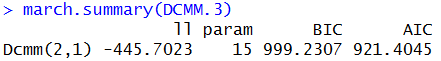
\includegraphics[scale=0.8]{dcmm_3}
    \caption{the summary of the DCMM with more hidden chains.}
    \label{fig:dcmm_3}
\end{figure}\newline
In the last example of DCMM the order of VC is raised to 2 and the order of the HC is reset to 1.
\begin{verbatim}
DCMM.4 <- march.dcmm.construct(PEWEE,orderHC=1,M=2,orderVC=2,maxOrder=3,
                               popSize=1,gen=1,iterBw=50,stopBw=0.0001)
march.summary(DCMM.4)
\end{verbatim}•
\refig{fig:dcmm_4} shows the summary. Of all examples this model has the best results with respect to the BIC, AIC and loglikelihood. 
\begin{figure}[h]
    \centering
    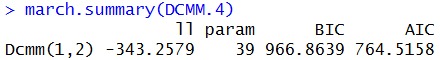
\includegraphics[scale=0.8]{dcmm_4}
    \caption{the summary of the DCMM with more visible chains.}
    \label{fig:dcmm_4}
\end{figure}\\
For the best fitting model (DCMM.4) the optimal sequence of hidden states should be extracted. This is occured with the usage of the viterbi algorithm. 
\begin{verbatim}
help(march.dcmm.viterbi)
HS <- march.dcmm.viterbi(DCMM.4,PEWEE)

print(HS)
print(PEWEE@y)
\end{verbatim}•
For further informations and a mathematical explanation of the viterbi algorithm read \cite{Forney1973} and \cite{Berchtold2002}

\subsection{Analysis of the hidden states}
To analyse the hidden states we use the example provided in the help page of the march.dcmm.construct() function. Therefore the HMM is built. 
\begin{verbatim}
help(march.dcmm.construct)
data(sleep)
HMM <- march.dcmm.construct(sleep,orderHC=1,orderVC=0,M=3,gen=1,
                            popSize=1,iterBw=10,stopBw=0.0001)
print(HMM)
\end{verbatim}
For the computation of the most likely sequences of the hidden states the Viterbi Algorithm is used. 
\begin{verbatim}
HS <- march.dcmm.viterbi(HMM,sleep)
\end{verbatim}•
Now the most likely sequence of hidden states is converted into a data frame using the following code with the for loop. 
\begin{verbatim}
HS2 <- matrix(NA,nrow=1000,ncol=7)
HS2 <- as.data.frame(HS2)
for (i in 1:1000){
  temp <- HS[[i]]
  ltemp <- length(temp)
  HS2[i,1:ltemp] <- temp
}
\end{verbatim}•
To visualize the hidden states the package TraMineR is required which already should be loaded. If not see the first chapter where it is described how to load a package. With the following code two plots are created.
\begin{verbatim}
hs.labels <- c("1", "2", "3")
hs.seq <- seqdef(HS2, alphabet=hs.labels, states = hs.labels,
							labels = hs.labels)

seqfplot(hs.seq, border = NA, title = "10 most frequent sequences")
seqdplot(hs.seq, border = NA, 
                title = "Distribution of hidden states by period")
help(seqplot)
\end{verbatim}•
 If the following error message appears, the plot window is not big enough. In R-Studio it is easy to size this window up.  
\begin{verbatim}
Error in plot.new() : figure margins too large
\end{verbatim}•
\subsection{Hierarchical Models}
In another example a strictly hierarchical model is created. Therefore we need seed model which is created with the code below. In fact it is an HMM first order. 
\begin{verbatim}
Seed.Model <- march.dcmm.construct(sleep,orderHC=1,orderVC=0,M=3,gen=1,
                                   popSize=1,iterBw=1,stopBw=0.0001)
print(Seed.Model)

HMM.h1 <- Seed.Model
\end{verbatim}•
Now a matrix for the high order transition probabilities between hidden states is used. Here called A  which is mathematical explained in \cite{Berchtold2002}
\begin{verbatim}
A <-  matrix(nrow=3,ncol=3,c(0.5,0.5,0,
                             0,0.5,0.5,
                             0,0,1),byrow=TRUE)
A
\end{verbatim}•
This matrix A is now used to calculate the next HMM with the usage of the seed model calculated before. 
\begin{verbatim}
HMM.h1@A <- A             
HMM.h1 <- march.dcmm.construct(sleep,orderHC=1,orderVC=0,M=3,gen=1,
                               popSize=1,iterBw=5,stopBw=0.0001,
                               seedModel=HMM.h1)
print(HMM.h1)
\end{verbatim}•
To extract the hidden state sequences the Viterbi Algorithm is taken. 
\begin{verbatim}
HS.h1 <- march.dcmm.viterbi(HMM.h1,sleep)
\end{verbatim}•
The triangular model calculated in the next step only differs from the model before only in the transition matrix between hidden states A. The seed model is the same model as calculated above so please make sure it has been built. 
\begin{verbatim}
HMM.h2 <- Seed.Model
A <-  matrix(nrow=3,ncol=3,c(0.5,0.25,0.25,
                             0,0.5,0.5,
                             0,0,1),byrow=TRUE)
A
HMM.h2@A <- A             
HMM.h2 <- march.dcmm.construct(sleep,orderHC=1,orderVC=0,M=3,gen=1,
                               popSize=1,iterBw=5,stopBw=0.0001,
                               seedModel=HMM.h2)
print(HMM.h2)
\end{verbatim}•
All this three different model calculations only differs in their transition matrix A which is shown in \refig{fig:A}.
\begin{figure}[h]
    \centering
    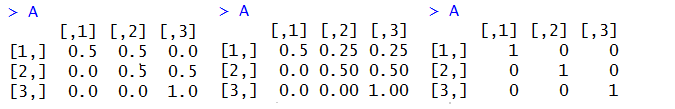
\includegraphics[scale=0.8]{Atri}
    \caption{The differences between the matrices A from left to right: first model, triangular model and classification model}
    \label{fig:A}
\end{figure}
For the classification the hidden state sequences are extracted.
\begin{verbatim}
HS.c <- march.dcmm.viterbi(HMM.c,sleep)
\end{verbatim}•
This is convertet into a data frame with the following code. 
\begin{verbatim}
HSc <- matrix(NA,nrow=1000,ncol=7)
HSc <- as.data.frame(HSc)
for (i in 1:1000){
  temp <- HS.c[[i]]
  ltemp <- length(temp)
  HSc[i,1:ltemp] <- temp
}
\end{verbatim}•
For this data frame a seqdef object is created with the help of the TraMineR package. Therefore the following code is necessary. 
\begin{verbatim}
Creation of a TraMineR seqdef object for the observed data
hs.labels.c <- c("0","1","2","3","4","5")
hs.c <- seqdef(sleep_df, alphabet=hs.labels.c, states = hs.labels.c,labels = hs.labels.c)

# Presentation of the data by group
seqfplot(hs.c, border = NA, group=HSc[,1],title = "25 most frequent sequences",tlim=1:25)
seqdplot(hs.c, border = NA, group=HSc[,1],title = "Distribution of observed data")
\end{verbatim}•
If the following error message appears, may the plot window is not big enough. In R-Studio it is easy to size this window up.  
\begin{verbatim}
Error in plot.new() : figure margins too large
\end{verbatim}•






